%% Change "letterpaper" in the following line to "a4paper" if you must.

\documentclass[10pt,letterpaper]{article}

\usepackage{cogsci}
\usepackage{pslatex}
\usepackage{apacite}
\usepackage{subcaption}
\usepackage{graphicx}
\usepackage{amsmath}
\usepackage{relsize}
\usepackage{natbib}
\usepackage{float}



\title{Learning Parallels: Emergence of Representation of Analogous Structure in Neural Networks}
 
\author{{\large \bf Andrew Lampinen (lampinen@stanford.edu)} \\
  Department of Psychology, Stanford University \\
  Jordan Hall, 450 Serra Mall, Stanford CA 94305 
  \AND {\large \bf Shaw Hsu (cshawhsu@stanford.edu)} \\
  Department of BioPhysics, Stanford University \\
  Varian Physics Building, 382 Via Pueblo Mall, Stanford CA 94305
  \AND {\large \bf James L. McClelland (mcclelland@stanford.edu)} \\
  Department of Psychology, Stanford University \\
  Jordan Hall, 450 Serra Mall, Stanford CA 94305} 


\begin{document}

\maketitle


\begin{abstract}
Neural networks have been shown to extract analogous structure from tasks which do not share inputs or outputs. This may explain the value of multi-task training, and also may underlie the power of human analogical reasoning. We generalize linear analysis techniques to explore the analogies extracted in non-linear networks, explore two tasks with non-overlapping structure and show that analogous structure is commonly extracted, and address the potential implications 

\textbf{Keywords:} 
neural networks; structure learning; representation; analogy; transfer; 
\end{abstract}


\section{Introduction}
Neural networks are capable of extracting analogous structure from knowledge domains that are completely non-overlapping in their inputs and outputs \citep{Hinton1986,Rogers2008}. This sets them apart from simple forms of statistical pattern recognition \citep{Rogers2008} such as linear data analysis techniques like PCA. However, there have been important theoretical developments in linear neural networks recently which have been shown to have applications to understanding learning in non-linear neural networks \citep{Saxe2013}. How can we employ the full power of non-linear neural networks while still gaining some value from linear analysis techniques? How and why do representations that reflect structural analogies in the environment emerge in neural networks? \par 
\subsection{Why Should We Care?}
Why might analogy extraction be important? Analogy is often considered a critical part of human cognition \cite[e.g.]{Gentner2003}, and forming representations which reflect analogous structures allows neural networks to form representations that support analogy \citep{Pennington2014,Kollias2013}. This may explain how analogies can emerge intuitively in the human mind instead of requiring the computationally expensive symbolic search often used in analogical processing systems \cite[e.g.]{Falkenhainer1989}. \par
More generally, multi-task learning has proven beneficial for producing efficient learning and effective generalization in neural networks on a variety of tasks, \cite[e.g.]{Dong2015,Rusu2015}. Even a small amount of learning on distinct but related tasks has been shown to improve performance, for example training a translation system not only on the main translation task, but also on image captioning and autoencoding \citep{Luong2016}. Learning on numerous language translation pairs can even give generalization without further training to unseen language pairs \citep{Johnson2016}. Because human experience is filled with distinct tasks that share common elements (language, various perceptual modalities, etc.) the way that structure is learned across tasks may be essential to understanding human intelligence and building better artificial intelligence systems.\par
However, we have little understanding of how, why, or when neural networks are able to extract ``hidden'' analogous structure like this. Here, we describe a preliminary investigation into this question, and in the process describe a new approach to analyzing neural network representations that may yield more general insights. 
\section{A Simple Task}
In the original work of \citet{Hinton1986}, a neural network was taught to answer queries about the structure of two perfectly analogous family trees (one English and one Italian), and was shown to generate representations that extract the analogy, in the sense that analogous people from different family trees are represented similarly. Here, we pare this task down to its barest essentials: two perfectly analogous domains with separate inputs and ouputs. For our task, the inputs can be thought of as the set of letters \(\{R,L,\rho,\lambda\}\), and the outputs as \(\{P,D,S,\pi,\delta,\sigma\}\). The task can be seen as mapping an input letter onto the letters that it can follow (e.g. ``R'' can follow ``D'' as in ``draw,'' but cannot follow ``S''), where there is an analogy between the Latin and Greek letters. See below for the input-output mapping: 
\[
\begin{array}{c|cccccc} 
& P & D & S & \pi & \delta & \sigma \\
\hline
R & 1 & 1 & 0 & 0 & 0 & 0 \\
L & 1 & 0 & 1 & 0 & 0 & 0 \\
\rho & 0 & 0 & 0 & 1 & 1 & 0\\
\lambda & 0 & 0 & 0 & 1 & 0 & 1\\
\end{array} 
\]
We train a neural network with a single hidden layer (4 units) to solve this task. (No biases were used, weights were initialized randomly between 0 and 0.1, all training was done by SGD with \(\eta = 0.01\) for 500 epochs.) We include only a single non-linearity (a rectifier) at the output layer. When and how does this simple network extract the analogous structure across the domains? \par
\begin{figure*}
\centering
\begin{subfigure}{0.22\textwidth}
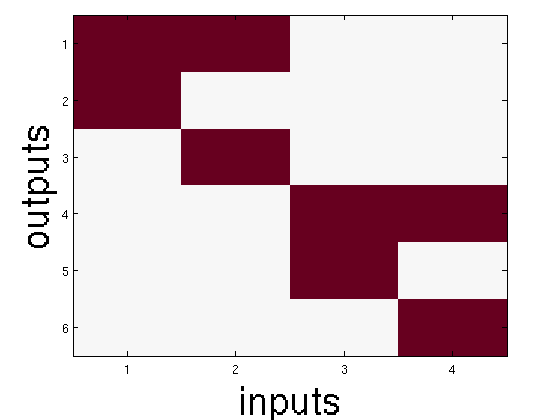
\includegraphics[width=\textwidth]{figures/nonlinear_IO.png}
\caption{$\Sigma_{IO,nl}$}
\end{subfigure}
\huge{$=$}
\begin{subfigure}{0.22\textwidth}
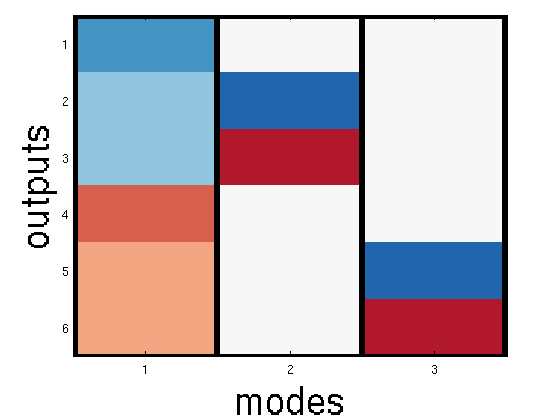
\includegraphics[width=\textwidth]{figures/U_nl.png}
\caption{$U_{nl}$}
\end{subfigure}
\LARGE{$\times$}
\begin{subfigure}{0.22\textwidth}
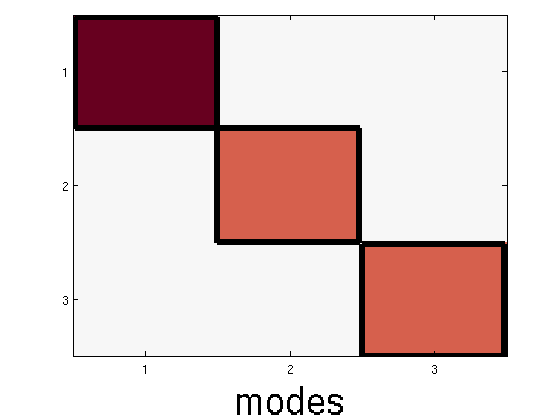
\includegraphics[width=\textwidth]{figures/S_nl.png}
\caption{$S_{nl}$}
\end{subfigure}
\LARGE{$\times$}
\begin{subfigure}{0.22\textwidth}
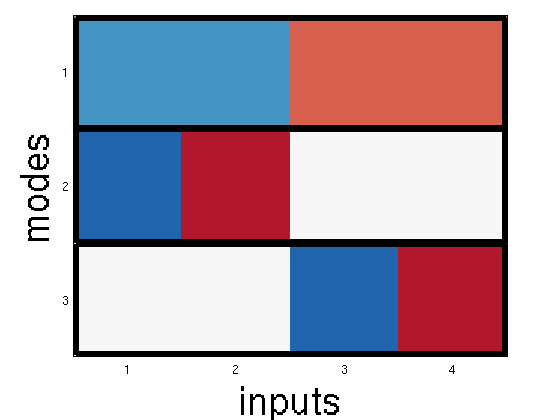
\includegraphics[width=\textwidth]{figures/V_nl.png}
\caption{$V_{nl}$}
\end{subfigure}
\caption{SVD of regular input-output correlation matrix (components with singular value zero are omitted from this figure)}
\label{regular_SVD_figure}
\end{figure*}
\subsection{Linear Analysis?}
As mentioned above, there have been recent developments in the theory of linear neural networks which show that the process of learning is entirely driven by the Singular Value Decomposition (SVD) of the input-output correlation matrix \citep{Saxe2013}. These results have been shown to have implications for the learning of non-linear networks as well, so linear neural networks can be thought of as a relaxation of non-linear neural networks that makes analysis more tractable. Thus one might ask whether our questions can be analyzed within this linear framework. \par
Unfortunately, linear networks cannot extract analogous structure from non-overlapping inputs and outputs. With non-overlapping inputs and outputs, the I/O correlation matrix is block diagonal, and the SVD modes will thus occur within blocks (see Fig. \ref{regular_SVD_figure} for demonstration of this on our task). In other words, the representational components that a linear network learns will be separated by domain, there will not be any sharing of structure across domains.\par 
Furthermore, the optimal rank $k$ approximation to a matrix is to take the top $k$ components from the SVD \citep{Mirsky1960}. If a linear network's hidden layers are restricted to rank lower than that of the input-output correlation matrix, detail within the domains will be lost. This means that a linear neural network cannot solve the task perfectly if any of its hidden layers has a number of units smaller than the rank of the input-output correlation matrix. In the usual case when the input-output correlation matrix is full rank, a linear network requires at least one unit for every output or one for every input, whichever is smaller. By contrast, a non-linear network can exploit the analogy between the domains to learn the task with fewer hidden units. In the next section, we outline an approach to analyzing this task based on reducing it to a linear problem.
\begin{figure*}
\centering
\begin{subfigure}{0.22\textwidth}
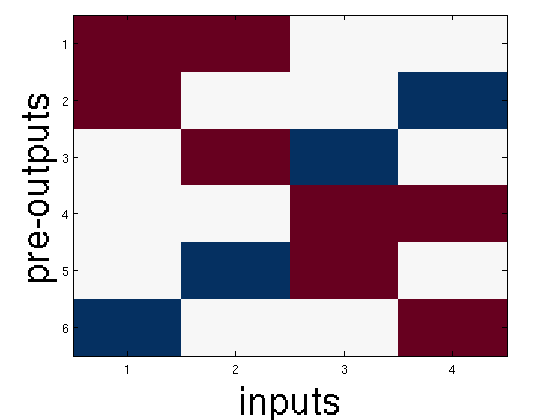
\includegraphics[width=\textwidth]{figures/linearized_IO.png}
\caption{$\Sigma_{IO,lz}$}
\end{subfigure}
\huge{$=$}
\begin{subfigure}{0.22\textwidth}
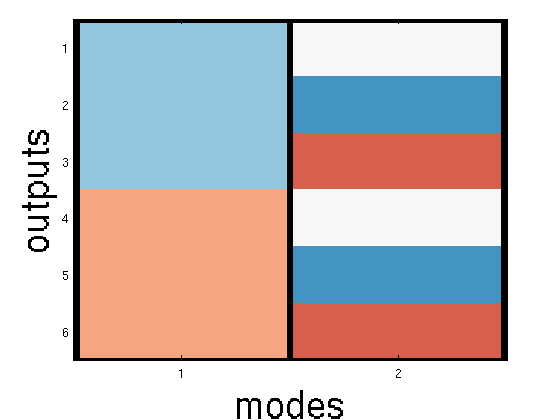
\includegraphics[width=\textwidth]{figures/U_lz.png}
\caption{$U_{lz}$}
\end{subfigure}
\LARGE{$\times$}
\begin{subfigure}{0.22\textwidth}
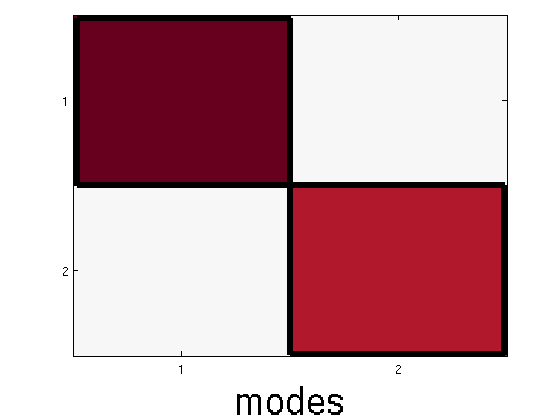
\includegraphics[width=\textwidth]{figures/S_lz.png}
\caption{$S_{lz}$}
\end{subfigure}
\LARGE{$\times$}
\begin{subfigure}{0.22\textwidth}
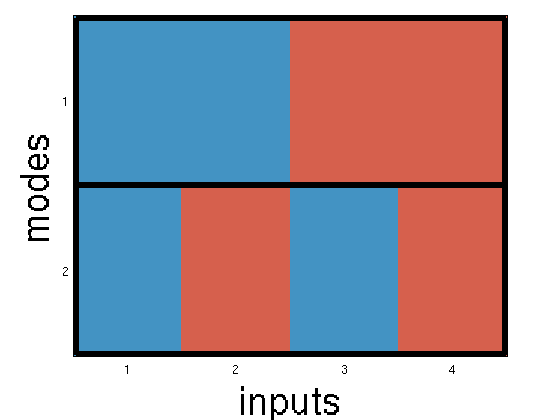
\includegraphics[width=\textwidth]{figures/V_lz.png}
\caption{$V_{lz}$}
\end{subfigure}
\caption{SVD of linearized input-output correlation matrix (components with singular value zero are omitted from this figure)}
\label{linearized_SVD_figure}
\end{figure*}
\subsection{A Linearized Approach}
\begin{figure}
\centering
\begin{subfigure}{0.5\textwidth}
\centering
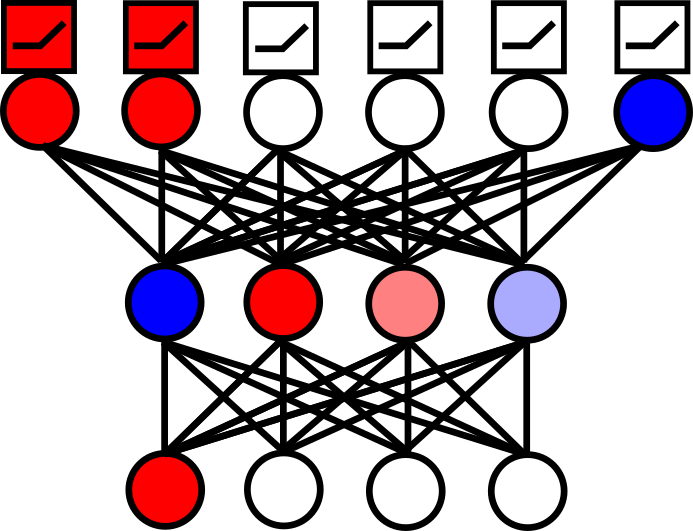
\includegraphics[width=0.5\textwidth]{figures/network_diagram.png}
\caption{Simple task, showing a sample propagation of an input through the network with the single non-linearity at the output.}
\label{network_diagram}
\vspace*{1em}
\end{subfigure}
\begin{subfigure}{0.5\textwidth}
\centering
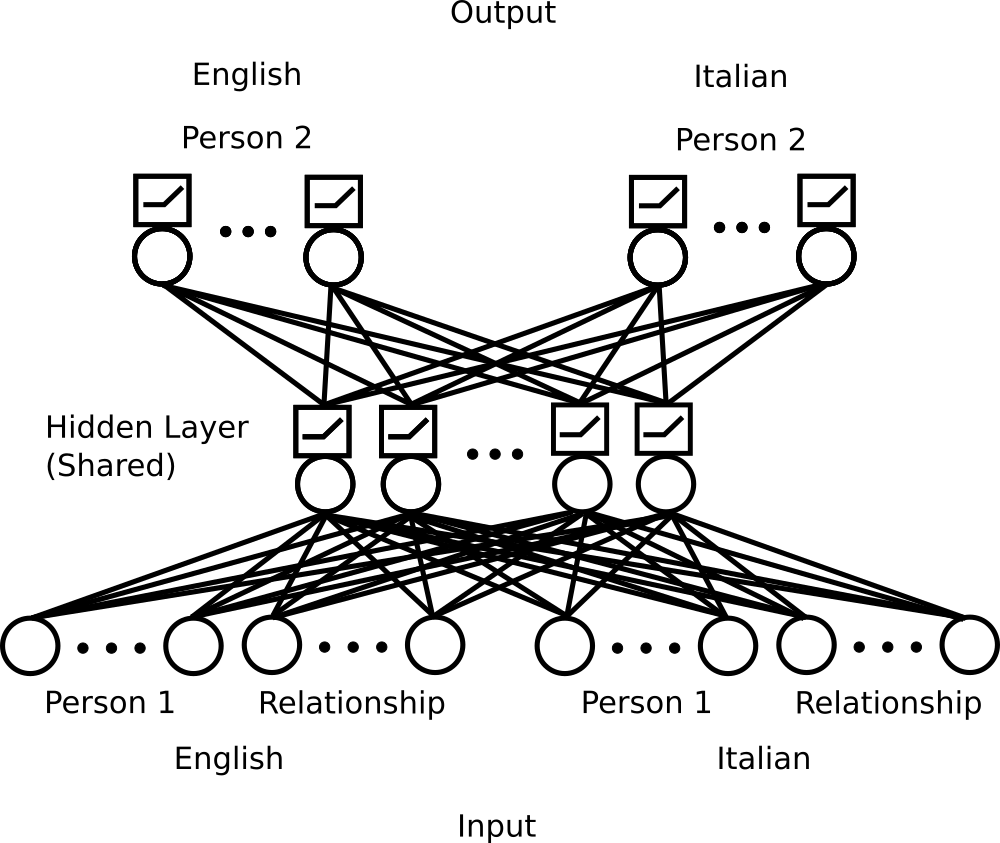
\includegraphics[width=0.8\textwidth]{figures/family_tree_network_diagram.png}
\caption{Family tree task}
\label{family_tree_network_diagram}
\end{subfigure}
\caption{Network Diagrams}
\end{figure}
Consider the fact that our task is solvable by logistic regression (i.e. it is linearly separable). Thus, while a linear network cannot extract the analogous structure from the task, inserting a single non-linearity after the output layer may cause it to do so again. In the case that the non-linearity is a sigmoid, this essentially reduces the problem to logistic regression; here we will use rectified linear units in our analysis because their structure makes the output patterns more intuitively interpretable. \par 
Once this almost-linear network has solved the problem, consider its outputs immediately prior to the non-linearity. These are produced by the linear part of the network, and together with the non-linearity suffice to produce the desired output pattern. We can use these to turn the problem into a linearly analyzable one -- simply treat these pre-nonlinearity outputs as outputs of a linear network. Then the problem becomes susceptible to the types of linear analyses discussed above. We will refer to this as the ``linearized'' version of the task. See fig. \ref{network_diagram} for a diagram of the network. \par 
In the simple task described above, the solution that the nonlinear network discovers the majority of the time (about 75\%) is to output the same pattern on both sets of output units, but offset the ``incorrect'' domain sufficiently negative so that the output after the rectifier is zero, thus transforming the input-output mapping into the linearized input-output mapping as follows:
{ \relsize{-1}
\[
\left[ \begin{matrix} 
1 & 1 & 0 & 0 & 0 & 0 \\
1 & 0 & 1 & 0 & 0 & 0 \\
 0 & 0 & 0 & 1 & 1 & 0\\
 0 & 0 & 0 & 1 & 0 & 1\\
\end{matrix}  \right] 
\mathlarger{\mathlarger{\Rightarrow}}
\left[ \begin{matrix} 
1 & 1 & 0 & 0 & 0 & -1 \\
1 & 0 & 1 & 0 & -1 & 0 \\
 0 & 0 & -1 & 1 & 1 & 0\\
 0 & -1 & 0 & 1 & 0 & 1\\
\end{matrix}  \right] 
\] }
(Note that the network can actually map the first element of one domain onto either element of the other, since they are perfectly symmetrical. This solution occurs as well, but we discuss the one shown here for clarity, the other solution amounts to just shuffling some rows and columns.) Now that we have a linearized version of the task, we can perform a linear analysis. When the SVD of this linearized I/O correlation matrix is evaluated, a rank 2 solution emerges. The components of the SVD of the linear portion of this solution can be qualitatively identified as: \begin{enumerate}
\item The separation of the domains
\item The analogous structure within the domains
\end{enumerate}
(see fig. \ref{linearized_SVD_figure}). The first component is similar to the first component of the regular SVD in that it reflects the separation of the domains, but the second component collapses the two components of the linear SVD. In other words, the analogy has been learned. Thus a network with a single non-linearity is able to represent the analogy by allowing the outputs in both domains to vary, and simply suppressing the output from the ``wrong'' domain for the current task.\par
Furthermore, because this solution is rank 2, a non-linear network with two hidden units should be able to solve the task, whereas a linear network will require at least 3. We have verified these results empirically for this task. Thus the ability of a non-linear neural network to extract common structure from multiple tasks can allow it to find lower-rank (i.e. more parsimonious) solutions. 
\subsection{Evolution of I/O Mappings}
%\begin{figure}
%\centering
%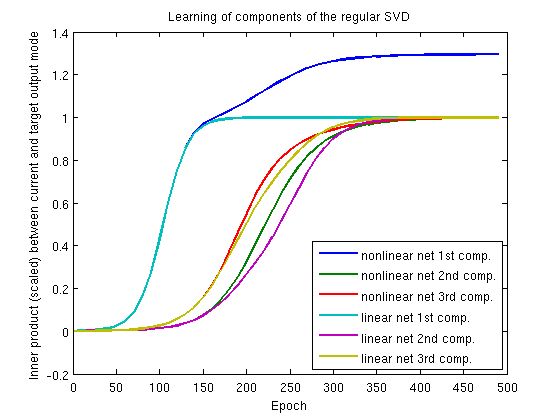
\includegraphics[width=0.5\textwidth]{figures/regular_SVD_component_learning.png}
%\caption{I/O SVD component learning (dot product between output mode of an SVD component and the response of the network to the corresponding input mode, scaled by the corresponding singular value)}
%\label{regular_SVD_component_learning}
%\end{figure}
%
%\begin{figure}
%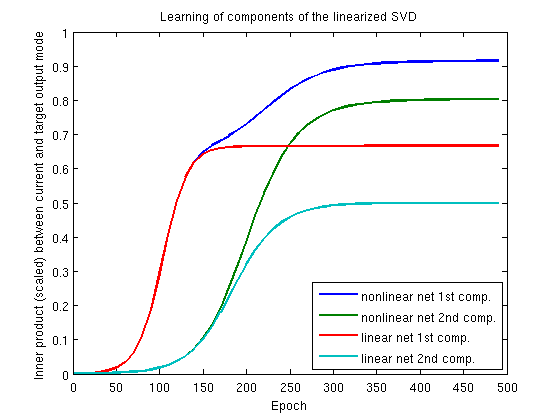
\includegraphics[width=0.5\textwidth]{figures/linearized_SVD_component_learning.png}
%\caption{Linearized I/O SVD component learning (dot product between output mode of an SVD component and the response of the network to the corresponding input mode, scaled by the corresponding singular value)}
%\label{linearized_SVD_component_learning}
%\end{figure}
Of course, there are a number of solutions that could potentially emerge in the non-linear network (such as just learning the mapping of each input to its output pattern independently), but on a set of 100 runs we conducted, shared structure was extracted on about 75\% of them (as measured by more than 20\% score on the below cross-projection metric). What drives this fairly consistent emergence of representations that reflect the analogous structure? In this section we consider the evolution of the representations and outputs over the course of learning on this simple task. \par 
The output structure of the network goes through a consistent progression, which we will first describe qualitatively in terms of the general structure of the input-output mapping at various epochs (the exact values depend on the vagaries of the initialization and training data order, so the matrices shown here are idealizations that are only accurate within about 0.1 on any given run). The outputs begin as small positive numbers, approximately 0 (because the weights are initialized uniformly between 0 and 0.1). Next, the network captures the base rate activations of each output unit (around epoch 75).
{ \relsize{-1}
\[ 
\text{base rates} = \left[ \begin{matrix} 
0.5 & 0.25 & 0.25 & 0.5 & 0.25 & 0.25 \\
\vdots & \vdots &\vdots &\vdots &\vdots &\vdots \\
 0.5 & 0.25 & 0.25 & 0.5 & 0.25 & 0.25\\
\end{matrix}  \right] 
\] 
}
Then the network captures the existence of the two domains but not the structure within them (around epoch 140). Up to this point, a linear network follows nearly the same learning trajectory.
{ \relsize{-1}
\[
\text{base rates by domain} = \left[ \begin{matrix} 
1 & 0.5 & 0.5 & 0 & 0 & 0 \\
1 & 0.5 & 0.5 & 0 & 0 & 0 \\
0 & 0 & 0 & 1 & 0.5 & 0.5  \\
0 & 0 & 0 & 1 & 0.5 & 0.5  \\
\end{matrix}  \right] 
\] 
}
Then it learns the internal structure of the domains (they are not learned at exactly the same time, which is learned first depends on the initilization). Finally around epoch 400 it has solved the task completely, with some sort of offset structure in the non-linear case, or without in the linear case:
{ \relsize{-1}
\[
\text{solution with offsets} = \left[ \begin{matrix} 
1 & 1 & 0 & 0 & 0 & -1 \\
1 & 0 & 1 & 0 & -1 & 0 \\
 0 & 0 & -1 & 1 & 1 & 0\\
 0 & -1 & 0 & 1 & 0 & 1\\
\end{matrix}  \right] 
\]
}
For most of the learning, it seems that the networks are extracting similar structure, so one might expect that even the linear network would show some representation of the analogy. Indeed, there is an interesting pattern to the results, wherein both the linear and non-linear networks begin to extract the analogy between the domains. See fig. \ref{SVD_cross_projection_learning} for a plot of how much each domain's input mode projects to the \textbf{other domain's} output mode, i.e. ``cross-talk'' between the domains. This measures the extent to which the network is extracting shared structure as the extent to which one domain cues the response of the other. While both networks develop some representation of the analogy initially, this activity extinguishes rapidly within the linear network, while it stabilizes at a positive value in the non-linear network. \par
\begin{figure}[H]
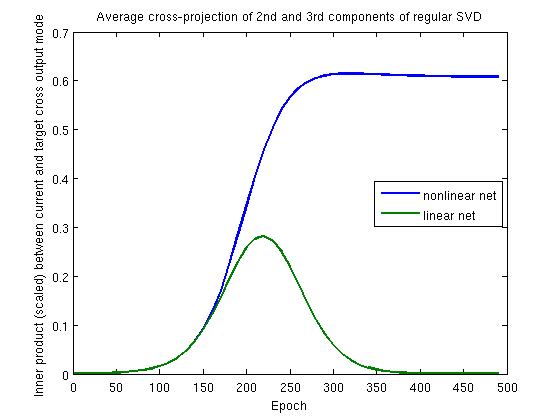
\includegraphics[width=0.45\textwidth]{figures/SVD_cross_projection_learning.png}
\caption{I/O SVD component cross-projection (dot product between output mode of an SVD component and the response of the network to the \textbf{other domain's} input mode)}
\label{SVD_cross_projection_learning}
\end{figure}
Why do both networks show some representation of the analogy initially? At the stage when the base rates by domain have been learned, adding a little bit of shared structure actually reduces MSE, e.g. in the below case the small increase in MSE from the \(\pm 0.1\) values is more than offset by the larger decrease from moving the 0.5 values closer to their true values 
{ \relsize{-1}
\[
\left[ \begin{matrix} 
1 & 0.6 & 0.4 & 0 & 0.1 & -0.1 \\
1 & 0.4 & 0.6 & 0 & -0.1 & 0.1 \\
0 & 0.1 & -0.1 & 1 & 0.6 & 0.4  \\
0 & -0.1 & 0.1 & 1 & 0.4 & 0.6  \\
\end{matrix}  \right] 
\] 
}
Indeed, suppose there is any hidden unit which responds differentially within the domains (as they all will to some extent because of the random initialization). Then the gradient of the output weights for this unit will naturally point in the direction of analogy extraction at this point. For example, if the unit responds positively to the first unit of each domain and negatively to the second, once the base rates have been learned the gradient of the output weights within each domain will be negative toward the second output and positive toward the third for that domain, and zero for the other domain's outputs' weights. When small updates in the direction of all of these gradients are made, since the unit responds to inputs from multiple domains, the updates will drive the network toward the pattern shown above. Thus exploiting this analogous structure enables the network to reduce error, even if it must eventually discard it in the linear case.  \par
Why does this structure persist in the non-linear network but die out in the linear network? In the linear network, as mentioned above, the optimal solution the network must reach is to precisely learn the linear SVD. Since the components of the linear SVD do not have shared structure, the linear network cannot represent analogous structure at convergence. By contrast, the non-linear network can simply offset the other domain's outputs further below zero, and thus make use of the analogy rather than being harmed by it. 
\section{Reanalyzing Hinton's Family Tree Example}
Next, we briefly turn our attention to the example of \citet{Hinton1986} which inspired this work. Hinton described a task of learning the structure of two isomorphic family trees, one English and one Italian (see fig. \ref{hinton_family_tree_figure}). This structure is presented implicitly in the form of presenting a person (e.g. ``Jennifer'') and a relationship (e.g. ``Father''), and training the network to produce the correct target person (``Andrew'' in this case). Unlike the simple problem above, this problem is not linearly separable, so we used a network with a non-linearity at the hidden layer as well. Hinton used the same relationship inputs for both families, but to highlight the extraction of analogous structure we separated these into distinct inputs (these could be thought of as corresponding to the English and Italian words for different relations, e.g. ``uncle'' vs. ``zio'' ). See fig. \ref{family_tree_network_diagram} for a diagram of our network. We trained this network using SGD with \(\eta = 0.005\) for 1000 epochs. \par 
Of course, in a task which requires multiple non-linearities, we cannot do as simple an analysis as in the earlier task. However, we can split the network up into layers, each of which has a single non-linearity at the output, and then perform an analysis like the above on each layer. In this way we can understand something about the computations that the network is performing and the structure it is extracting. However, the interpretation will not be as simple as in the single layer case. \par
\begin{figure}[H]
\centering
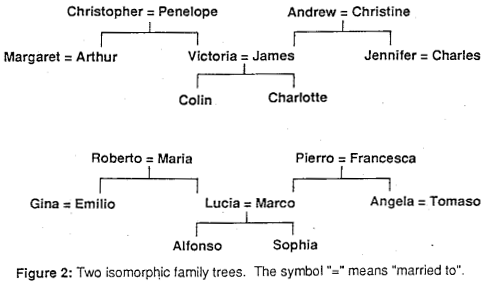
\includegraphics[width=0.45\textwidth]{figures/hinton_family_tree_figure.png}
\caption{Family trees from \citet{Hinton1986}, (permission pending).}
\label{hinton_family_tree_figure}
\end{figure}
\vspace{-2em}
\begin{figure}[H]
\centering
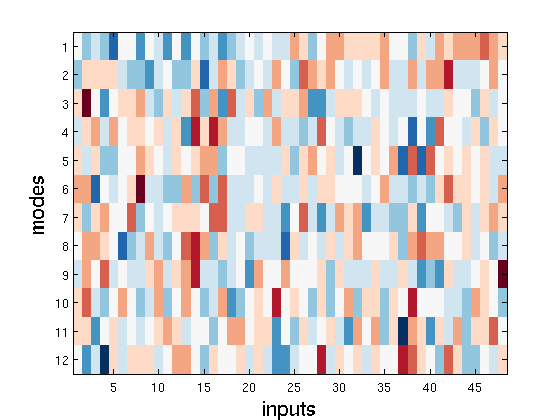
\includegraphics[width=0.5\textwidth]{figures/ft_input_mode_example.png}
\caption{Example layer 1 SVD input modes from the family tree task}
\label{ft_input_mode_example}
\end{figure}
\vspace{-2em}
\begin{figure}[H]
\centering
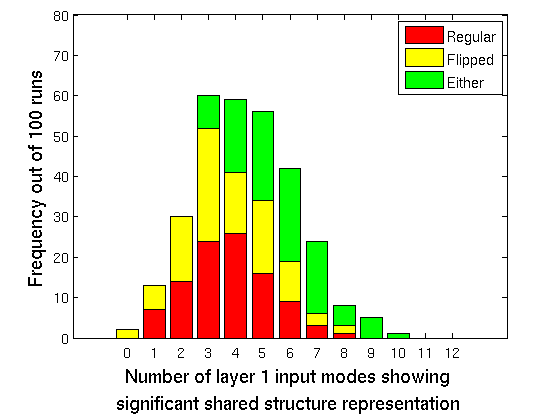
\includegraphics[width=0.5\textwidth]{figures/ft_input_mode_significance_hist.png}
\caption{How many of the input modes from the layer 1 SVD showed significantly more projection than would be expected between the domains regularly, if one family tree was completely flipped, or projected significantly onto either one (without double counting)}
\label{ft_input_mode_sig_hist}
\end{figure}
This difficulty is compounded by the complexity of the structure being learned in each family (see fig. \ref{ft_input_mode_example} for an example of the first layer input mode structure one network learned). In the simple problem above it was possible to ``eyeball'' the structure extraction, but here the structure is too rich. There are a variety of possible ways the families can be mapped onto one another (e.g. flipping the tree left to right and swapping all genders), and it's possible that the networks are extracting overlapping structure from several of these analogies. In this setting, how can we examine whether the network is learning the analogy? \par
As a first test of the analogous structure extraction, we examined the evidence for it in the input modes of the first layer SVD. To do this, we computed the dot product of the mode's weights for one family with that mode's weights for the other family, and then tested the significance of this similarity by comparing it to the chance distribution generated nonparametrically by randomly permuting the columns of the input mode matrix 1000 times and computing the same dot product for each of these. We denoted a mode as showing significant extraction of the analogy if it showed a stronger similarity between the weights for the two families' inputs than 95\% of the random permutations of that mode did. \par
We repeated this process across 100 network initilizations and found a great deal of analogous structure was being extracted. The runs had a median of 4 modes showing significant analogous structure extraction, and all the runs had at least one mode with significant analogous structure extraction (for comparison, if 5\% of the modes showed significant results by chance, we would still expect 54\% of the runs to yield no significant results, and the median number of shared structure components would thus be zero). To account for the symmetry of the tree under flipping, we repeated the same analysis after permuting the second families input columns in such a way as to effectively flip the family tree and reverse all the genders. Since the network has no way to distinguish between the ``regular'' mapping and this ``flipped'' mapping during learning, we would expect to see a similar frequency of modes which reflect the analogy with this flipped structure, and indeed the distribution is similar. Furthermore, the runs had a median of 6 modes showing significant extraction of the analogy to either the regular or flipped mapping, in 95\% of the runs the network had extracted 3 or more significant componentsfrom at least one of the mappings, and in all of the runs it had extracted 3 or more components that significantly represent one analogy or the other (if we assume 5\% false positives again, we would expect results this extreme in only 0.01\%, 4\% and 3\% of the runs, respectively). See fig. \ref{ft_input_mode_sig_hist} for a histogram of the number of significant input modes by run for the different mappings. Clearly a great deal of analogous structure is being extracted in the layer 1 mapping. \par
We performed a similar analysis for the output modes of layer 2, and again found a great deal of analogous structure extraction, though less than in the input modes of the first layer. The median number of modes that showed significant analogous structure extraciton from either domain was 4, and in 64\% of the runs the network had extracted 3 or more significant components for the regular mapping or 3 or more significant components for the flipped mapping. It is somewhat unsurprising that the output mappings would show less shared structure extraction than the input mappings, since to solve the task the network must offset any shared structure in the output modes to prevent it appearing in the output. \par  
We have not analyzed in detail the modes projecting into or out of the hidden layer -- we leave that for future work. Nevertheless, we think these results provide insight about the degree and type of extraction of the analogy occuring on this task. Extraction of analogous structure is both common and general (in the sense that the networks are extracting structure corresponding to several different analogies between the domains, even within the same network).
\section{Disussion}
We have explored how a simple neural network can extract the analogy between multiple tasks with non-overlapping inputs and outputs. We showed that a single non-linearity at the output layer of a neural network can allow the network to represent this common structure on a simple task, and that it emerges naturally (even in a linear network) once the base rates of the various domains have been learned, because incorporating it reduces MSE. A linear network must discard this analogy to reach its optimal solution, but a non-linear network is able to retain it by simply offsetting the outputs to a sufficiently negative value for its nonlinearity, and does so the majority of the time (75\%). Here we used rectifiers as our non-linearity, but the same solution type is achievable with sigmoid, tanh, etc. \par 
We then broadened our approach to explore the family tree task originally proposed in \citet{Hinton1986}. Because this task is not linearly separable, we created a general network with two nonlinear layers, and applied our analysis to each layer. We found evidence of a great deal of extraction of two possible analogies between the families in the network (either the intended isomorphism between the family trees, or one in which one family tree was flipped and the gender of its members was flipped), and that networks seemed generally to be discovering elements of both analogies. Indeed, the shared structure extraction seemed even more common than in the simpler task above, while on the simple task 25\% of the networks showed no evidence of common structure extraction, on the family tree task every network extracted at least three components that projected significantly onto one analogy or the other. \par 
These results suggest that rather than an advanced cognitive ability requiring symbolic computations, analogy may be simply a natural feature of gradient based learning in nonlinear neural networks. It is particularly interesting to think about how analogical learning between tasks can facilitate more rapid learning and better performance on these tasks, as with the multi-task machine learning examples cited above. More broadly, the power and generality of human cognition may result from the range of deeply related tasks we engage in, all of which we can extract analogous structures from. 
\subsection{Future Directions}
We think there are a variety of exciting future directions suggested by this work. 
\begin{enumerate}
\item It would be useful to explore how learning trajectories might change with explicit cueing of the analogy (e.g. presenting analogous exemplars together), or when one domain is learned before another. How does this change extraction of analogous structure?
\item Similarly, how does structure extraction change when some inputs are shared between analogous items (as \citet{Hinton1986} did with the relationship inputs) and can thus act as cues to similarity?
\item What happens when structures do not perfectly match, as is the case in most real world analogies?
\item When and why is analogous structure not extracted -- what features of the initilization cause this, and how does it interact with task complexity?
\item It would be interesting to think more broadly about the role that this structure extraction could play in analogical reasoning in human cognition, possibly serving in effect as a form of automatic amortized inference about potential analogical relationships.
\item Finally, in our analysis of the family tree task we analyzed the input modes of the first layer and the output modes of the second layer. An important future direction would be exploring the modes which map into and out of the hidden layer, and what they imply about the representations generated at the hidden layer. This would also allow us to apply this analysis to deep networks with more than a single hidden layer.
\end{enumerate}
\section{Acknowledgments}
This material is based upon work supported by the National Science Foundation Graduate Research Fellowship under Grant No. DGE-114747.
\bibliographystyle{apacite}

\setlength{\bibleftmargin}{.125in}
\setlength{\bibindent}{-\bibleftmargin}

\bibliography{shared_reps}


\end{document}
